\documentclass[main]{subfiles}
\begin{document}

\section*{Lecture 11 // Sept 29 // Instanton Floer Homology}
\addcontentsline{toc}{section}{Lecture 11 -- Instanton Floer Homology}

The rest of the course will follow this general outline.
\begin{enumerate}
\item Broad overview of Instanton Floer Homology
\item Formal properties \& applications
\item More detailed discussion of (1)
\item More recent papers
\end{enumerate}

Instanton Floer Homology is a $3$-manifold invariant. Originally, it was defined only for integer homology spheres, and we'll restrict to $Y$ a $\mathbb{Z}\mathrm{HS}^3$ for simplicity, but the constructions we'll discuss can be extended.

The general procedure is as follows:
\[
Y \rightsquigarrow C(Y) \rightsquigarrow H_\ast(C(Y)),
\]
\[
\mathbb{Z}\mathrm{HS}^3 \qquad \text{Instanton chain complex} \qquad \text{Instanton Floer homology}.
\]

Where does $C(Y)$ come from? Two slogans:
\begin{enumerate}
\item $\infty$-dimensional Morse homology associated to the CS functional, i.e., there is a mysterious $S^1$-valued functional on an auxiliary space associated to $Y$ (like $\mc{A}/\mc{G}$, but for $Y^3$):
\[
\CS : \mc{A}/\mc{G} \longrightarrow \mathbb{R}/\mathbb{Z}.
\]
Whenever you have an $\mathbb{R}$-valued function, we take the Morse homology:
\begin{itemize}
\item the critical points of CS become the generators of the chain complex,
\item the differentials are defined (roughly) by studying the gradient flow of CS.
\end{itemize}
\item The generators of $C(Y)$ are in correspondence with conjugacy classes of $\SU(2)$ representations of $\pi_1(Y)$. So $C(Y)$ actually comes from $\pi_1$.
\end{enumerate}

Today, we'll broadly discuss (1) \& (2), and why they're the same.

\subsection*{What is the Chern-Simons Functional}

Take $Y^3$ a $\mathbb{Z}\mathrm{HS}^3$ (though nothing today depends on that). Fix an $\SU(2)$ bundle over $Y$. Since $c_2(Y)=0$, there's only one such bundle, the trivial one $E = Y\times\mathbb{C}^2 \to Y$.

Just like before, we study $\mc{A} = \{\SU(2) \text{ connections on } E\}$ and $\mc{G}\curvearrowright \mc{A}$, $\mc{G} = \Gamma(\Aut(E))$. Since $E$ is trivial, $\mc{G} \cong \Maps(Y,\SU(2))$.

Note that $\pi_0(\mc{G})\cong \mathbb{Z}$, since $\SU(2)\cong S^3$, and maps $Y\to S^3$ are determined by the degree $\deg(g)\in \mathbb{Z}$.

$\mc{A}/\mc{G}$ = configuration space / gauge, the domain of CS.

\begin{definition}
The Chern-Simons Functional is a map
\[
\CS : \mc{A}/\mc{G} \longrightarrow S^1, \qquad \CS(A) = \frac{1}{8\pi^2}\int_Y \tr\left(A\wedge dA + \frac{2}{3}A\wedge A\wedge A\right).
\]
\end{definition}

By this, we mean first: fix a global trivialization of $E$. In this global trivialization, $\nabla$ is represented by a matrix of $1$-forms $A$, which is the input of the integral.

\begin{exercise}
If $g\in\mc{G}$ is a global gauge transformation, $\CS(g^\ast A) = \CS(A) + \deg(g)$.
\end{exercise}

This gives another way of saying that $\pi_0(\mc{G})\cong \mathbb{Z}$; each connected component corresponds to a trivialization, so this is saying that, up to homotopy, there are $\mathbb{Z}$-many trivializations of $E$. The value of the Chern-Simons Functional depends on which trivialization you choose. This definition is super explicit but not as insightful as the following alternate definition.

\begin{definition}
Let $A$ be a connection on $E$. Choose any:
\begin{itemize}
\item smooth $4$-manifold $W^4$ such that $\partial W\cong Y$,
\item $\SU(2)$-bundle $E_W$ on $W$ such that $E_W|_Y \cong E$,
\item $\SU(2)$-connection $\nabla_W$ such that $\nabla_W|_Y = \nabla$.
\end{itemize}
Then $\CS(\nabla) = \dfrac{1}{8\pi^2}\displaystyle\int_W \tr(F_{\nabla_W}\wedge F_{\nabla_W})$.
\end{definition}

\begin{center}
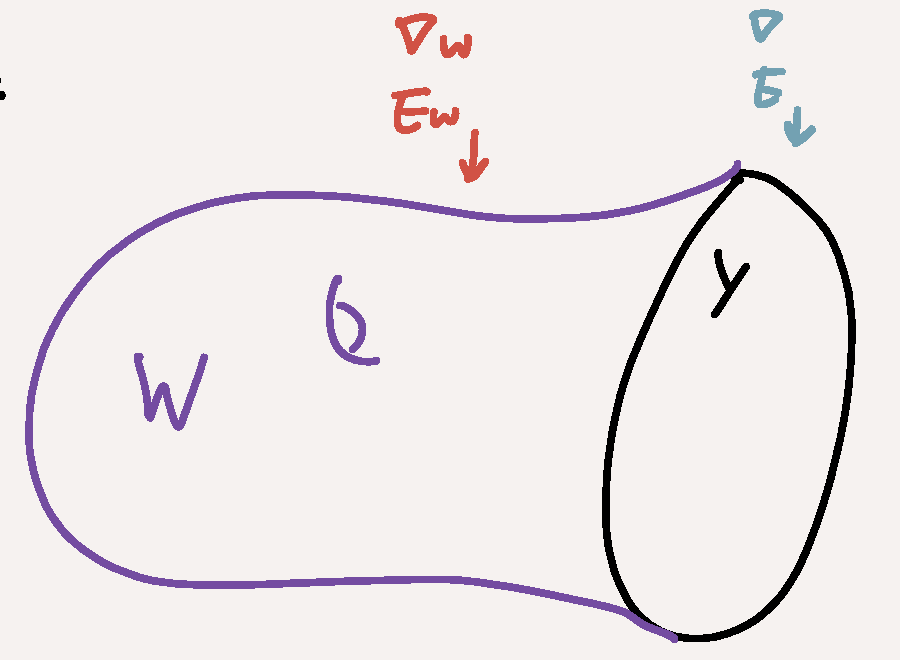
\includegraphics[width=0.4\linewidth]{figures/fig_lec11_cobordism1.png}
\end{center}

This definition follows from the definition of relative characteristic classes. But as-is, you should be skeptical that this is well defined. Let's choose a different $W'$, $E_{W'}$, $\nabla'$. Then
\[
\CS(\nabla) = \frac{1}{8\pi^2}\int_W \tr(F_{\nabla_W}\wedge F_{\nabla_W}) \quad \text{and} \quad \CS(\nabla) = \frac{1}{8\pi^2}\int_{W'} \tr(F_{\nabla_{W'}}\wedge F_{\nabla_{W'}}).
\]
If this definition is well-defined, then $\CS(\nabla)-\CS(\nabla') = 0$. To compute the difference, glue $W$ and $-W'$ along $Y$ to get an $\SU(2)$ bundle over a closed $4$-manifold.

\begin{center}
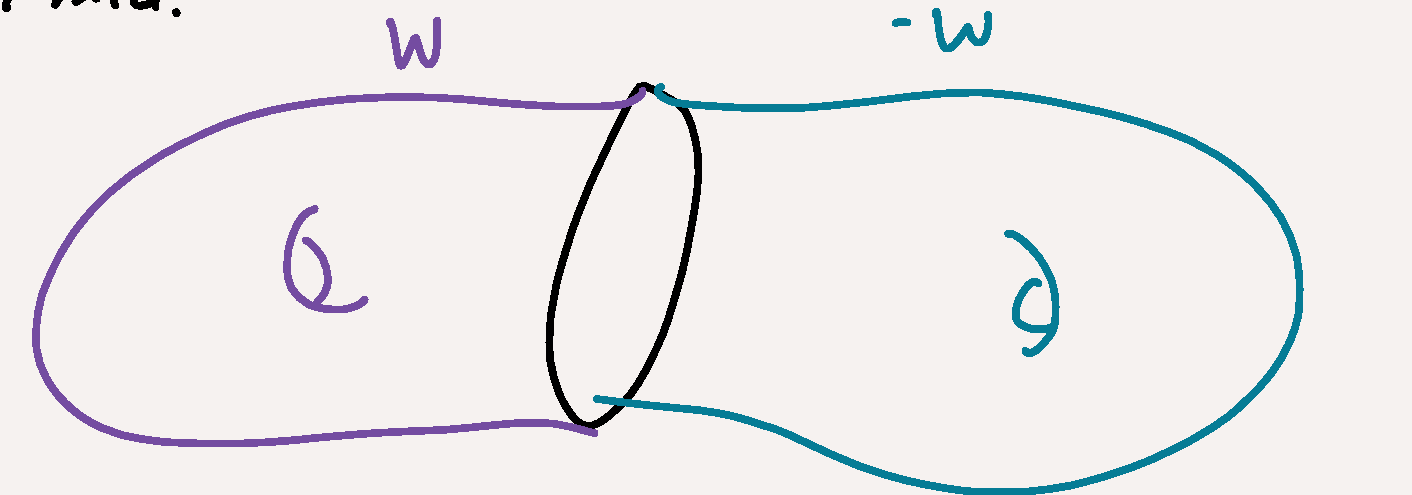
\includegraphics[width=0.45\linewidth]{figures/fig_lec11_gluing.png}
\end{center}

Then their difference becomes an element of $\mathbb{Z}$:
\[
\frac{1}{8\pi^2}\int_W \tr(F_{\nabla_W}\wedge F_{\nabla_W}) - \frac{1}{8\pi^2}\int_{W}\tr(F_{\nabla_{W'}}\wedge F_{\nabla_{W'}}) = \left\langle c_2(E_\Sigma), [W\cup_Y -W']\right\rangle \in \mathbb{Z}.
\]
Thus different $W$'s change $\CS(\nabla)$ by an integer, so $\CS(\nabla)$ is well-defined in $S^1$.

\begin{remark}
The bundles $E_W, E_{W'}$ over $W$ and $W'$ glue together to a well-defined bundle $E_\Sigma$ over $W\cup_Y -W'$. The same is true for $\nabla_W$ and $\nabla_{W'}$, obtaining $\nabla_\Sigma$. The Chern-Simons integral of this connection is that of a closed $4$-manifold.
\[
\CS(\nabla_\Sigma) = \frac{1}{8\pi^2}\int_{W\cup_Y -W'}\tr(F_{\nabla_\Sigma}\wedge F_{\nabla_\Sigma}) \in \mathbb{Z},
\]
and splits as $\displaystyle\int_W \tr(F_{\nabla_\Sigma}|_W\wedge F_{\nabla_\Sigma}|_W) - \int_{W'}\tr(F_{\nabla_\Sigma}|_{W'}\wedge F_{\nabla_\Sigma}|_{W'})$.
\end{remark}

However, for the connections $\nabla_W$ and $\nabla_{W'}$ over $4$-manifolds with non-empty boundary, $\CS(\nabla_W)\notin \mathbb{Z}$. In our proof of well-definedness, we relied on some gluing procedure without verifying what that procedure actually is: this was incredibly sloppy. We should also ask whether this definition plays well with $\mc{G}$.

In order to glue $E_W$ and $E_{W'}$ together, we must fix identifications $E_W|_Y \cong E_{W'}|_Y$. Since there is only one $\SU(2)$ bundle over $Y$, the trivial one, we could argue that $E_W, E_{W'}$ are trivial bundles, thus $E_\Sigma$ is trivial, so the difference is zero. While the first part of this is true, like we saw with $\mathbb{CP}^1$, two trivial bundles could be glued via some nontrivial boundary map, like $\mathbb{Z}^n$, which results in a nontrivial bundle. Even simpler, two trivial $\mathbb{R}$-bundles over the interval $I$ could be glued via a twist, resulting in the M\"obius band. The number of these different maps is the number of retrivializations of the bundle on the boundary. So we must ask: how many retrivializations of $\nabla_W$ are there? The answer is $\mathbb{Z}$, as we saw earlier, and these $\mathbb{Z}$-many gluings give $\mathbb{Z}$-many $\SU(2)$ bundles over $W$!

\begin{claim}
Re-trivializing a bundle $E_W$ over $\partial W\cong Y$ by composing with some $g\in\mc{G}$ changes $c_2(E_\Sigma)$ by $\deg g \in \mathbb{Z}$.
\end{claim}

\begin{lemma}
The two definitions agree.
\end{lemma}

\begin{proof}
This follows immediately from Stokes' theorem: $\left(\displaystyle\int_W d\beta = \int_{\partial W}\beta\right)$.
\[
8\pi^2 \CS(A) = \int_Y \tr\left(A\wedge dA + \frac{2}{3}(A\wedge A\wedge A)\right) = \int_W d\left(\tr\left(A\wedge dA + \frac{2}{3}(A\wedge A \wedge A)\right)\right).
\]
Simplifying,
\[
d\left(\tr\left(A\wedge dA + \frac{2}{3}(A\wedge A\wedge A)\right)\right) = \tr\left(d(A\wedge dA) + \frac{2}{3}d(A\wedge A\wedge A)\right)
\]
\[
= \tr\left(dA\wedge dA - A\wedge d^2 A + \frac{2}{3}\left(dA\wedge A\wedge A - A\wedge dA\wedge A + A\wedge A\wedge dA\right)\right)
\]
\[
= \tr\left(dA\wedge dA + \frac{2}{3}dA\wedge A\wedge A - \frac{2}{3}A\wedge dA\wedge A + \frac{2}{3}A\wedge A\wedge dA\right)
\]
\[
= \tr(dA\wedge dA + 2\, dA\wedge A\wedge A) = \tr(dA\wedge dA + dA\wedge A\wedge A + A\wedge A\wedge dA)
\]
\[
= \tr\big((dA+A\wedge A)\wedge(dA+A\wedge A)\big) + \tr(A\wedge A\wedge A\wedge A) = \tr(F_A\wedge F_A),
\]
since $\tr(A\wedge A\wedge A\wedge A) = 0$. Thus
\[
\int_Y \tr\left(A\wedge dA + \frac{2}{3}(A\wedge A\wedge A)\right) = \int_W \tr(F_A\wedge F_A) = 8\pi^2\left\langle c_2(E_\Sigma), [W\cup_Y -W']\right\rangle. \qedhere
\]
\end{proof}

\begin{remark}
Timeline: this all happened pre-Donaldson, post relative characteristic classes.
\end{remark}

Just like in Donaldson's theorem, we want to study the critical points of CS, which we'll denote by $\Crit(\CS)\subset \mc{A}/\mc{G}$. What about interpretation \#2?

\begin{theorem}
$\nabla \in \mc{A}/\mc{G}$ is a critical point of the Chern-Simons functional iff $\nabla$ is flat, i.e., $F_A=0$.
\end{theorem}

\begin{proof}
\[
\nabla \in \Crit(\CS) \iff \left.\frac{d}{dt}\right|_{t=0} \CS(\nabla+tb) = 0 \iff \left.\frac{d}{dt}\right|_{t=0} 8\pi^2\CS(\nabla+tb) = 0
\]
\[
\iff \int_Y \tr\left((A+tb)\wedge d(A+tB) + \frac{2}{3}\big((A+tb)\wedge(A+tb)\wedge(A+tb)\big)\right) = 0
\]
Using $d(A+tB) = dA\wedge B - A\wedge dB$,
\[
\iff \int_Y \tr\left(B\wedge dA + A\wedge dB + \frac{2}{3}B\wedge A\wedge A + \frac{2}{3}A\wedge B\wedge A + \frac{2}{3}A\wedge A\wedge B\right) = 0
\]
\[
\iff \int_Y \tr(2B\wedge dA + 2B\wedge A\wedge A) = 0 = 2\int_Y \tr(B\wedge F_A) = 0 \quad \forall B
\]
\[
\iff F_A = 0.
\]
\[
\grad_A \CS = \ast F_A. \qedhere
\]
\end{proof}

\begin{theorem}
Critical points of the Chern-Simons functional modulo gauge are in bijection with $\SU(2)$ representations of $\pi_1(Y)$ modulo conjugation.
\end{theorem}

\begin{definition}
The character variety of a $3$-manifold is
\[
R(Y) = \{\SU(2) \text{ representations of } \pi_1(Y)\}/\!\sim,
\]
where $\rho_0 \sim \rho_1$ iff $\rho_1 = g^{-1}\cdot \rho_0 \cdot g$.
\end{definition}

In this language, $\Crit(\CS) \leftrightarrow R(Y)$. We now prove the theorem.

\begin{proof}
Taking the holonomy gives a map
\[
\{\text{flat connections}\} \to \{\SU(2) \text{ representations of } \pi_1(Y)\}.
\]
Since $\hol^{g^\ast(\nabla)}_p(\gamma) = g_p^{-1}\circ \hol^\nabla_p(\gamma)\circ g_p$, this holonomy descends to a map on the quotient
\[
\{\text{flat connections}\}/\mc{G} \to \{\SU(2) \text{ representations of } \pi_1(Y)\}/\!\sim \ = R.
\]

It's not obvious this map is surjective. To show surjectivity, let $\rho : \pi_1(Y) \to \SU(2)$ be a representation of $\pi_1(Y)$. Construct an $\SU(2)$ bundle $E$ and connection $\nabla$ on $E$ as follows:
\begin{enumerate}
\item Form $\widetilde{E} = \widetilde{Y}\times \mathbb{C}^2$, the trivial bundle over the universal cover of $Y$.
\item Quotient out $\widetilde{E}$ by identifying the fibres $p\times \mathbb{C}^2$ and $\tau(p)\times \mathbb{C}^2$ for $\tau\in \Deck(\widetilde{Y})\cong \pi_1(Y)$ via the matrix given by $\rho(\gamma)\in \SU(2)$, where $\gamma\in\pi_1(Y)\leftrightarrow \tau$ between $p,\tau(p)$ (where $\gamma$ lifts to $\tau$).
\end{enumerate}

\begin{center}
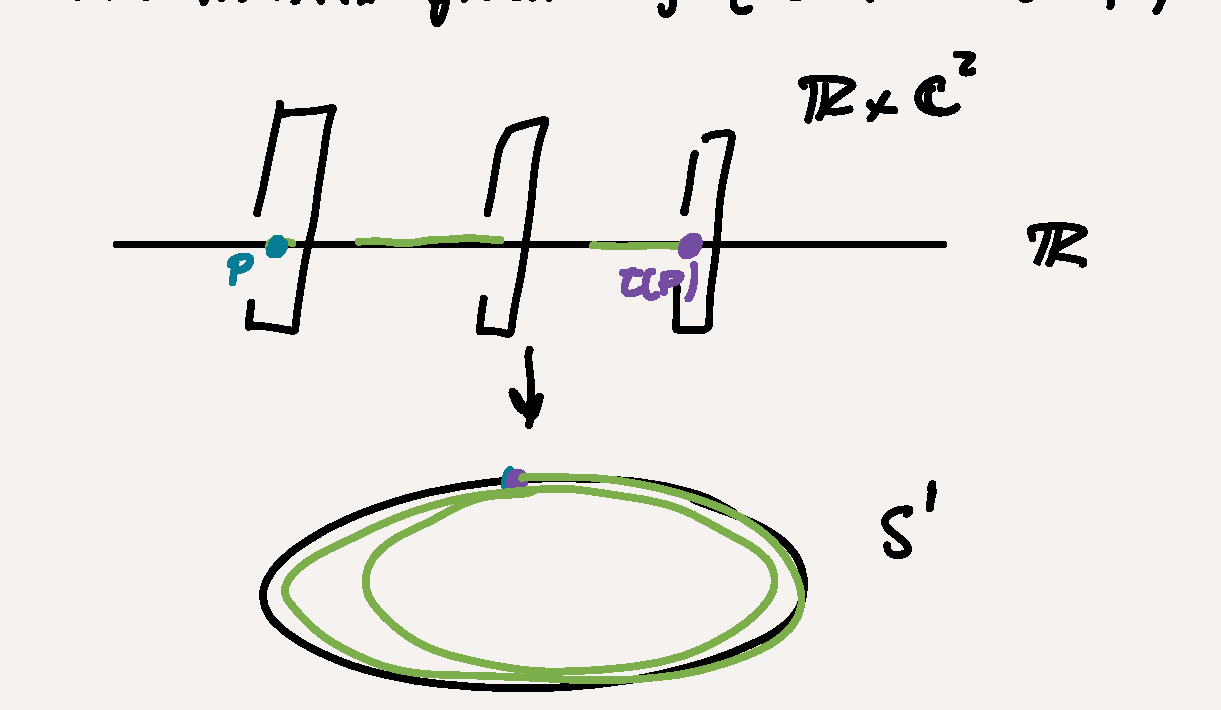
\includegraphics[width=0.75\linewidth]{figures/fig_lec11_fiber_quotient.png}
\end{center}

This defines a bundle $E$ over $Y$, as well as parallel transport on $E$ by pushing down parallel transport on $\widetilde{E}$. By construction, this parallel transport will have holonomy $\rho$. This shows surjectivity.
\end{proof}

\end{document}
